\documentclass[conference]{IEEEtran}
% \IEEEoverridecommandlockouts
% The preceding line is only needed to identify funding in the first footnote. If that is unneeded, please comment it out.
\usepackage{cite}
\usepackage{amsmath,amssymb,amsfonts}
\usepackage{algorithmic}
\usepackage{graphicx}
\usepackage{textcomp}
\usepackage{xcolor}
\usepackage{mathtools}
\def\BibTeX{{\rm B\kern-.05em{\sc i\kern-.025em b}\kern-.08em
T\kern-.1667em\lower.7ex\hbox{E}\kern-.125emX}}
\begin{document}

    \title{Evaluating Compile-Time Specialization For Entity-Component-System Implementations\\
    {\footnotesize }
    \thanks{}
    }

    \author{\IEEEauthorblockN{Wachirawich Kanil}
    \IEEEauthorblockA{\textit{Department of Computer Engineering} \\
    \textit{Chulalongkorn University}\\
    Bangkok, Thailand \\
    email address or ORCID}
    \and
    \IEEEauthorblockN{Tapaneeya Odmung}
    \IEEEauthorblockA{\textit{Department of Computer Engineering} \\
    \textit{Chulalongkorn University}\\
    Bangkok, Thailand \\
    email address or ORCID}
    \and
    \IEEEauthorblockN{Pranesh Ingkanunt}
    \IEEEauthorblockA{\textit{Department of Computer Engineering} \\
    \textit{Chulalongkorn University}\\
    Bangkok, Thailand \\
    email address or ORCID}
    \and
    \IEEEauthorblockN{Rangsiman Jearuksa}
    \IEEEauthorblockA{\textit{Department of Computer Engineering} \\
    \textit{Chulalongkorn University}\\
    Bangkok, Thailand \\
    email address or ORCID}
    }

    \maketitle

    \begin{abstract}
        The Entity-Component-System (ECS) pattern is widely used for applications in interactive systems,
        machine learning, and digital simulation contexts.
        From examining existing infrastructure and development tools and comparing to theoretical ECS models,
        we identified opportunities to reduce runtime overhead and increase performance through increased compile-time specialization.
        We present a framework implementing the ECS pattern and built upon C++ that aggressively applies compile-time
        metaprogramming techniques to reduce overhead.
        To analyze the potential of this approach, the framework was evaluated in comparison with
        industry-standard ECS libraries EnTT and Bevy ECS in terms of performance, executable size, and memory usage.
        The results showed that the presented implementation exhibited performance comparable to existing frameworks while
        substantially improving program size at a small cost to memory usage.
    \end{abstract}

    \begin{IEEEkeywords}
        Entity Component System, ECS, Data-Oriented Design, Software Architectures
    \end{IEEEkeywords}


    \section{Introduction}
    \label{sec:introduction}

    Entity-component-system (ECS) is a software architectural pattern used in interactive systems development,
    system simulations, and even machine learning.
    Its mechanisms are characterized by the entities, composed of components of data,
    and the systems which operate upon those components.
    An entity's behavior emerges from the systems that operate on its components, whether by mutating, adding, or removing these components.

    ECS has been implemented and used widely in production contexts.
    One of the more popular implementations is EnTT~\cite{ValtoLibraries_EnTT}, a header-only C++ library for game programming.
    This library has been used to develop many game titles, a major one of which is the Bedrock edition of Minecraft.~\cite{mojang_minecraft_attribution}
    Another popular implementation is Bevy ECS~\cite{Bevy_Engine}, a data-driven game engine built in Rust, which was
    used in~\cite{machine-learning-bevy} to implement a machine learning solution.

    However, existing ECS implementations generally balance runtime flexibility with compile-time optimization in different ways.
    Many use runtime component registration, type-erased execution, runtime scheduling, or other dynamic mechanisms to support extensibility,
    while using templates to optimize frequently executed operations such as query building.
    As a result, compile-time specialization is often applied selectively rather than uniformly across all ECS subsystems.

    This work explores and investigates the extent of compile-time specializations that can be applied within an ECS implementation.
    We create a custom framework to evaluate its impact on core ECS functionalities while maintaining an interface suitable for practical software development.
    We then assess the resulting performance of this framework through benchmarking in comparison to existing production frameworks.


    \section{Related Work}
    \label{sec:related-work}

    EnTT is a modern C++ ECS library that uses compile-time optimization through extensive use of template metaprogramming.
    Component views, registries, and queries are expressed as template types, allowing the compiler to generate specialized
    implementations for each combination of component types.
    This eliminates virtual dispatch, enables aggressive function inlining, and dead code elimination, producing
    highly optimized iteration code with minimal runtime overhead.
    EnTT's approach leverages C++'s static type system to shift most of the ECS abstraction cost from runtime to compile time.

    Bevy ECS, written in Rust, achieves compile-time optimization by relying on Rust's generic type system and monomorphization.
    Systems declare the components they access through generic query types, and the compiler generates specialized code for each query at compile time.
    Rust's ownership and borrowing rules also provide compile-time guarantees about aliasing and mutability, allowing
    the LLVM to safely optimize memory accesses and eliminate unnecessary runtime checks.
    The resultant code is efficient and statically typed with strong safety guarantees and performance comparable to handwritten loops.

    Unity's Data-Oriented Technology Stack (DOTS)~\cite{Unity_DOTS} combines compile-time code generation with the Burst compiler to maximize ECS performance.
    The Entities package~\cite{unity_entities}, part of DOTS, provides the ECS implementation.
    Entity queries are analyzed using C\# source generators, which produce specialized iteration code before compilation.
    The Burst compiler then compiles this generated code into highly optimized native machine code.
    DOTS also performs static analysis of system dependencies to construct efficient execution schedules,
    minimizing runtime scheduling overhead.
    The combination of all these optimizing factors resulted in a formidable engine for use with the classic game engine.

    \section{Design}
    \label{sec:design}

    We decided to implement our custom ECS framework using C++20 as it provides mature support for template
    metaprogramming, concepts, \verb|constexpr| evaluation, and deep type inference support.
    Additionally, it provides fine-grained control over memory layout and data locality.
    This made it well-suited for expressing ECS storage, systems execution, and query semantics as compile-time constructs.

    A crucial decision we had to make was choosing the type of component storage, as the selection greatly affects performance under varying scenarios.
    Two widely used types of ECS component storage are archetype-based and sparse-set-based storage.
    Cox, Williams, Vickers, Ward, and Headleand's work~\cite{cox2025run} showed that archetypes excel at large-scale entity iteration while sparse-sets are more efficient with component insertion and removal.
    We decided on sparse-set storage for the custom implementation to more conveniently support our optimization work.

    When implementing our framework, we applied three types of compile-time specialization:

    \begin{enumerate}
        \item \textbf{Component Storage:} We used template specialization on the component storage such that the data type could be derived and components registered at compile time.
        \item \textbf{System Registration:} We applied concepts to restrict the type of systems that are valid for the framework.
        Then, we applied compile-time template specialization over the function traits to derive the correct component types it requires.
        If the connected component storage did not have the required components, a compile-time error would be raised.
        By adjusting the order of system registration with the ECS, we could specify the system execution order in sequential order through loop unrolling.
        \item \textbf{Query Construction:} With compile-time loop unrolling and template folding over component types, we could generate query builder functions that exactly matched related component types.
    \end{enumerate}


    \section{Evaluation}
    \label{sec:method}

    For each framework, the size of the final executable is obtained by measuring the executable with the device's File Explorer.
    The memory usage of each framework is obtained by recording the Memory column from the Processes tab within the device's Task Manager while the benchmark was executing under steady-state conditions.

    The execution time of each ECS implementation was measured by recording the time immediately before and after
    the execution of all user-defined systems within one frame.
    For Bevy, we used Rust's \verb|Instant| to record timestamps.
    For EnTT and our implementation, we used the \verb|std::chrono::steady_clock| from C++.
    Unrelated plugins, rendering, and other external factors were excluded to isolate the frame execution time such that
    it served as a reliable primary performance metric.

    Four benchmark scenarios were designed to evaluate the frameworks under different workloads.
    For each scenario, the behavior and resultant work of user-defined systems remained equivalent across all frameworks.
    Benchmarks involving entity creation and destruction were designed to maintain a steady-state workload by ensuring
    that the ECS world returned to an equivalent state after each frame.
    While each framework differed in implementation details, care was taken to ensure computational work performed by
    the systems remained identical.
    This allowed a direct comparison of runtime performance between implementations.

    All benchmarks were compiled using release optimization settings, albeit with different compilers.
    The Bevy implementation was built using Rust's \verb|cargo --release| configuration.
    The EnTT implementation used the MinGW Release configuration, whereas our implementation was built
    using the MSVC Release configuration.

    Before measurements were recorded, each benchmark was allowed to execute for a warm-up period to reduce the
    influence of initialization overhead.
    Following this, execution time was recorded over 1,000 consecutive frames and written to a log file.
    The collected samples were then analyzed to compute the average execution time for each benchmark configuration.

    All tests were executed on local hardware using the same machine and operating environment to ensure consistency across measurements.
    The hardware specifications are as follows:

    \begin{itemize}
        \item CPU: 11th Gen Intel(R) Core(TM) i7-11800H @ 2.30 GHz
        \item GPU: Intel(R) UHD Graphics
        \item Memory: 3200 MHz 16.0 GB RAM
        \item Operating System: Windows 10 Version 22H2 (OS Build 19045.6466)
    \end{itemize}


    \section{Benchmark Suite}
    \label{sec:benchmark-suite}

    The benchmark suite was designed to exercise common ECS operations individually,
    including sequential iteration, entity creation and destruction, sparse component access, and archetype transitions.
    By isolating these behaviors into separate scenarios, differences between implementations can be attributed
    to specific aspects of ECS execution.

    \subsection{Entity Iteration}
    \label{subsec:entity-iteration}

    This benchmark evaluated the performance of sequential entity iteration in the ECS framework.
    The goal was to isolate the performance of entity traversal and component access.
    Configurations specified the entity count ranging from 1,000 to 64,000 to compare the scalability of entity iteration.

    For this benchmark, we emulated the behavior of a 2-dimensional physics engine which adjusts an entity's position according to their velocity.
    We defined the components $\mathbf{Pos} \mapsto \mathbb{R}^2$
    and ${\mathbf{Vel} \mapsto \mathbb{R}^2}$.
    The system query was defined as $\mathrm{Q}_\mathrm{S} = \mathrm{Q}(\mathbf{Pos}, \mathbf{Vel})$.
    Lastly, the user system was defined as $\mathrm{S}(\Delta t) = \left[\forall e \in \mathrm{Q}_\mathrm{S} : e.\mathbf{Pos} \leftarrow e.\mathbf{Pos} + e.\mathbf{Vel} \Delta t\right]$.

    Before each configuration, the specified number of entities were created and initialized with
    $\mathbf{Pos} \in \left\{ [-100, 100]^2 \right\}$ and $\mathbf{Vel} \in \left\{[-10, 10]^2\right\}$.
    The distribution of the random initialization was uniform.

    \subsection{Sparse Access}
    \label{subsec:sparse-access}

    This benchmark evaluated the performance of systems querying sparse entity archetypes in the ECS framework.
    The ratio of entities of interest to total entities will be referred to as the sparse ratio $R_s$.
    By varying the sparse ratio, the query-forming efficiency of ECS frameworks under sparse scenarios could be compared.

    For this benchmark, we emulated the behavior of a system that interacts with only entities of interest.
    In this implementation, entities of interest rotate their positions around the origin.
    We used components $\mathbf{Pos} \mapsto \mathbb{R}^2$ and $\mathbf{Int} \mapsto \varnothing$.
    The system query was defined as $\mathrm{Q}_\mathrm{S} = Q(\mathbf{Pos}, \mathbf{Int})$.
    Lastly, the user system was defined as $\mathrm{S} = \left[\forall e \in \mathrm{Q}_\mathrm{S} : e.\mathbf{Pos} \leftarrow \mathrm{Rot}(e.\mathbf{Pos}) \right]$ where $\mathrm{Rot} : \mathbb{R}^2 \rightarrow \mathbb{R}^2, \quad (x,y) \mapsto (y,-x)$.

    Before each configuration, the set number of 32,000 entities was created and initialized with $\mathbf{Pos} \in \left\{ [-100, 100]^2 \right\}$.
    A random subset of the total entities with size $R_s \times \mathrm{Entity Count}$ were then attached with $\mathbf{Int}$ corresponding to the sparseness configuration.
    The distribution of the random initialization was uniform.

    \subsection{Entity Creation and Destruction}
    \label{subsec:entity-creation-and-destruction}

    This benchmark evaluated the performance of the ECS framework when creating and destroying entities while running user-defined systems.
    To maintain a steady state throughout the benchmark, we set entity creation and destruction to the same rate $E$.
    In this benchmark, we adjusted the entity rate between configurations on a range from 32 to 2048.

    For this benchmark, we emulated the behavior of a system that creates entities and removes them after their duration has expired.
    We defined components $\mathbf{Life} \mapsto \mathbb{Z}$ and the system query $\mathrm{Q}_\mathrm{S} = \mathrm{Q}(\mathbf{Life})$.
    The user systems are separated into the entity creation system $\mathrm{C} = \left[\varnothing : \text{spawn }E\text{ entities with }\mathbf{Life \mapsto 2} \right]$
    and the entity destruction system $\mathrm{D}$, which is defined as follows.

    \[
        \left[
            \forall e \in \mathrm{Q}_\mathrm{S} :
            \left.
                \begin{cases}
                    e.\mathbf{Life} \leftarrow e.\mathbf{Life} - 1 & \text{if }e.\mathbf{Life} > 1 \\
                    \text{destroy }e & \text{otherwise.}
                \end{cases}
            \right.
        \right]
        \tag{1}\label{eq:benchmark-3-entity-destruction-system}
    \]

    The configuration did not prepare entities on initialization of the setup.

    \subsection{Structural Changes}
    \label{subsec:structural-changes}

    This benchmark evaluated the performance of ECS frameworks under workloads requiring heavy structural changes.
    This included the adding and removing of components, the changing of entity archetypes, and the change in queried entities.
    While the number of components remained static, we vary the number of entities in the configuration on a range from 100 to 8000 entities to scale the workload.

    For this benchmark, we emulated a system that operated a binary counter.
    If the bit on the counter is set, the system would attach the corresponding component, and vice versa.
    We defined the number component $\mathbf{Num} \mapsto \mathbb{Z}$, the counter bit components $\mathbf{B}_i \mapsto \varnothing \text{ for } i \in \left\{ 0, 1, \dots, 7 \right\} $
    and the system query $\mathrm{Q}_\mathrm{S} = \mathrm{Q}(\mathbf{Num})$.

    The system for this benchmark is a more complex process.
    Let $\mathrm{O}_i$ and $\mathrm{P}_i$ be operations on an entity $e$.
    $\mathrm{O}_i$ will attach $\mathbf{B}_i$ to $e$ if $e$ did not have the component and the binary representation of $e.\mathbf{Num}$ is $1$ in its $i$th digit.
    $\mathrm{P}_i$ will detach $\mathbf{B}_i$ to $e$ if $e$ had the component and the binary representation of $e.\mathbf{Num}$ is $0$ in its $i$th digit.
    To put simply, $\mathrm{O}_i$ and $\mathrm{P}_i$ updates the component based on the entity's $\mathbf{Num}$ value.
    We can then define the system $\mathrm{S} = \left[\forall e \in \mathrm{Q}_\mathrm{S} : \text{Apply }\mathrm{O}_i(e), \mathrm{P}_i(e)\text{ for } i \in \left\{ 0, 1, \dots, 7 \right\} \right]$


    \section{Results}
    \label{sec:results}

    \paragraph*{Entity Iteration}Table~\ref{tab:results-benchmark-1} shows the results of benchmark~\ref{subsec:entity-iteration}.
    From the benchmark output, we normalized the mean frame time by taking the ratio with the entity count for that configuration, and plotting this value yielded Fig.~\ref{fig:chart1}.
    This benchmark demonstrated that all three ECS frameworks exhibited the expected linear scaling for the simple data mutation system.
    EnTT incurred significantly higher costs at higher entity counts, implying larger per-entity iteration costs compared to the other frameworks.
    Bevy showed greater constant overhead, which was clear at lower entity counts, but scaled significantly better as entity count grew.
    This could be attributed to Bevy's archetype storage, which allowed for faster iteration compared to sparse-set storage.

    The custom implementation consistently exhibited the lowest frame times up to 8,000 entities, after which Bevy took over.
    The specialization and compiler optimizations used by the custom implementation allowed it to
    perform well when compared to EnTT.

    \begin{figure}
        \centerline{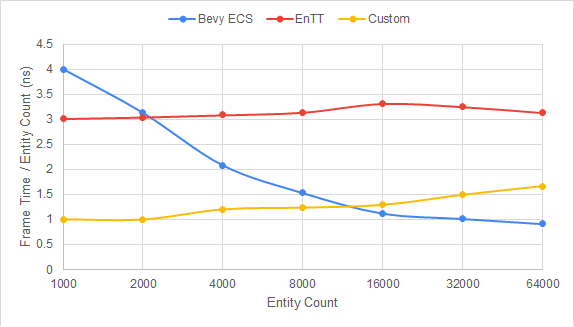
\includegraphics[width=0.4\textwidth]{chart1}}
        \caption{Benchmark~\ref{subsec:entity-iteration}: Scatter plot detailing frame time per entity as entity count increases.}
        \label{fig:chart1}
    \end{figure}

    \begin{table}[htbp]
        \caption{Benchmark~\ref{subsec:entity-iteration} – Statistics}
        \begin{center}
            \begin{tabular}{|c|c|c|c|c|c|}
                \hline
                \textbf{Entity} & \textbf{ECS} & \multicolumn{4}{|c|}{\textbf{Frame Time (microseconds)}} \\
                \cline{3-6}
                \textbf{Count} & \textbf{Framework} & \textbf{Mean} & \textbf{\textit{Std.Dev.}} & \textbf{\textit{Min}} & \textbf{\textit{Max}} \\
                \hline
                1000           & Bevy               & 3.994         & 1.547                      & 2                     & 23                    \\
                & EnTT               & 3.013         & 0.113                      & 3                     & 4                     \\
                & Custom             & 1.009         & 0.130                      & 1                     & 4                     \\
                \hline
                2000           & Bevy               & 6.254         & 1.514                      & 3                     & 17                    \\
                & EnTT               & 6.087         & 0.577                      & 6                     & 16                    \\
                & Custom             & 2.014         & 0.117                      & 2                     & 3                     \\
                \hline
                4000           & Bevy               & 8.333         & 1.041                      & 5                     & 17                    \\
                & EnTT               & 12.352        & 3.057                      & 12                    & 24                    \\
                & Custom             & 4.823         & 1.012                      & 4                     & 27                    \\
                \hline
                8000           & Bevy               & 12.264        & 2.136                      & 9                     & 38                    \\
                & EnTT               & 25.120        & 1.471                      & 23                    & 54                    \\
                & Custom             & 9.912         & 1.266                      & 9                     & 28                    \\
                \hline
                16000          & Bevy               & 18.002        & 2.766                      & 14                    & 59                    \\
                & EnTT               & 53.033        & 11.039                     & 49                    & 225                   \\
                & Custom             & 20.695        & 2.946                      & 19                    & 55                    \\
                \hline
                32000          & Bevy               & 32.512        & 2.912                      & 26                    & 44                    \\
                & EnTT               & 104.087       & 9.449                      & 100                   & 220                   \\
                & Custom             & 47.701        & 6.843                      & 43                    & 87                    \\
                \hline
                64000          & Bevy               & 58.591        & 4.719                      & 51                    & 88                    \\
                & EnTT               & 200.677       & 23.302                     & 184                   & 480                   \\
                & Custom             & 106.292       & 13.066                     & 94                    & 187                   \\
                \hline
            \end{tabular}
        \end{center}\label{tab:results-benchmark-1}
    \end{table}

    \paragraph*{Sparse Access}Table~\ref{tab:results-benchmark-2} shows the results of benchmark~\ref{subsec:sparse-access}.
    Plotting the mean frame time against the sparse ratio of the benchmark configuration yields Fig.~\ref{fig:chart2}.

    Considering the figure, we observe that while EnTT performed worse at high sparse ratios compared to the other frameworks,
    it exhibited superior efficiency when entities of interest are sparse, specifically at sparse ratio 0.1 and less.
    Bevy and the custom implementation showed similar decreases as entity density lowered, but the custom implementation had
    more constant overhead compared to Bevy.
    As such, the custom framework consistently underperformed in terms of sparse access efficiency compared to
    the other frameworks.

    \begin{figure}
        \centerline{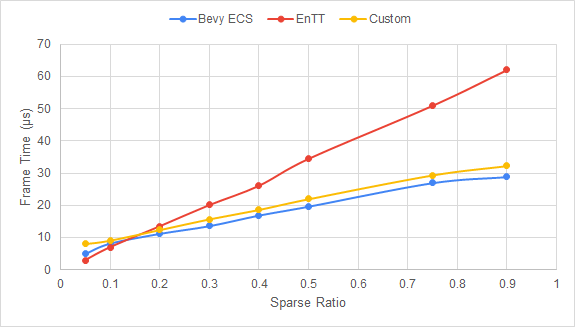
\includegraphics[width=0.4\textwidth]{chart2}}
        \caption{Benchmark~\ref{subsec:sparse-access}: Scatter plot detailing frame time at varying sparse ratios.}
        \label{fig:chart2}
    \end{figure}

    \begin{table}[htbp]
        \caption{Benchmark~\ref{subsec:sparse-access} – Statistics}
        \begin{center}
            \begin{tabular}{|c|c|c|c|c|c|}
                \hline
                \textbf{Sparse} & \textbf{ECS} & \multicolumn{4}{|c|}{\textbf{Frame Time (microseconds)}} \\
                \cline{3-6}
                \textbf{Ratio} & \textbf{Framework} & \textbf{Mean} & \textbf{\textit{Std.Dev.}} & \textbf{\textit{Min}} & \textbf{\textit{Max}} \\
                \hline
                0.90           & Bevy               & 28.845        & 3.830                      & 24                    & 55                    \\
                & EnTT               & 61.977        & 8.337                      & 58                    & 253                   \\
                & Custom             & 32.293        & 6.049                      & 29                    & 130                   \\
                \hline
                0.75           & Bevy               & 26.963        & 2.453                      & 21                    & 37                    \\
                & EnTT               & 50.910        & 9.785                      & 47                    & 255                   \\
                & Custom             & 29.378        & 5.894                      & 26                    & 76                    \\
                \hline
                0.50           & Bevy               & 19.676        & 2.164                      & 15                    & 33                    \\
                & EnTT               & 34.422        & 5.370                      & 32                    & 118                   \\
                & Custom             & 21.970        & 4.134                      & 20                    & 79                    \\
                \hline
                0.40           & Bevy               & 16.914        & 1.967                      & 13                    & 31                    \\
                & EnTT               & 26.063        & 1.767                      & 25                    & 53                    \\
                & Custom             & 18.633        & 3.173                      & 17                    & 58                    \\
                \hline
                0.30           & Bevy               & 13.631        & 1.741                      & 10                    & 33                    \\
                & EnTT               & 20.087        & 1.079                      & 19                    & 35                    \\
                & Custom             & 15.705        & 3.475                      & 14                    & 59                    \\
                \hline
                0.20           & Bevy               & 11.244        & 1.597                      & 8                     & 27                    \\
                & EnTT               & 13.517        & 3.530                      & 13                    & 69                    \\
                & Custom             & 12.363        & 2.294                      & 11                    & 65                    \\
                \hline
                0.10           & Bevy               & 8.211         & 1.489                      & 5                     & 28                    \\
                & EnTT               & 7.032         & 0.441                      & 6                     & 13                    \\
                & Custom             & 9.065         & 0.507                      & 9                     & 19                    \\
                \hline
                0.05           & Bevy               & 4.977         & 1.353                      & 3                     & 25                    \\
                & EnTT               & 3.004         & 0.063                      & 3                     & 4                     \\
                & Custom             & 8.011         & 1.018                      & 7                     & 39                    \\
                \hline
            \end{tabular}
        \end{center}\label{tab:results-benchmark-2}
    \end{table}

    \paragraph*{Entity Creation and Destruction}Table~\ref{tab:results-benchmark-3} shows the results of benchmark~\ref{subsec:entity-creation-and-destruction}.
    We normalized the mean frame time by taking the ratio with the entity rate for that configuration, and plotting this value yielded Fig.~\ref{fig:chart3}.
    For this benchmark, we observe EnTT and the custom framework exhibiting similar performance behavior, remaining relatively consistent as entity rate varied.
    Bevy, at low entity rates, showed a significant performance drop with frame times at multiples of the other frameworks.
    As entity rates increase, Bevy recovered from the static performance overhead, but not to comparable performance.

    \begin{figure}
        \centerline{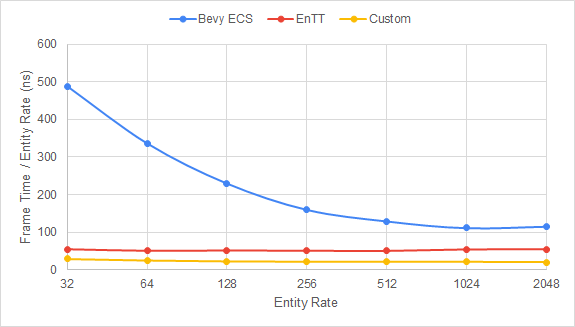
\includegraphics[width=0.4\textwidth]{chart3}}
        \caption{Benchmark~\ref{subsec:entity-creation-and-destruction}: Scatter plot detailing frame time per entity at varying entity rates.}
        \label{fig:chart3}
    \end{figure}

    \begin{table}[htbp]
        \caption{Benchmark~\ref{subsec:entity-creation-and-destruction} – Statistics}
        \begin{center}
            \begin{tabular}{|c|c|c|c|c|c|}
                \hline
                \textbf{Entity} & \textbf{ECS} & \multicolumn{4}{|c|}{\textbf{Frame Time (microseconds)}} \\
                \cline{3-6}
                \textbf{Rate} & \textbf{Framework} & \textbf{Mean} & \textbf{\textit{Std.Dev.}} & \textbf{\textit{Min}} & \textbf{\textit{Max}} \\
                \hline
                32            & Bevy               & 13.683        & 3.027                      & 8                     & 35                    \\
                & EnTT               & 1.060         & 0.237                      & 1                     & 2                     \\
                & Custom             & 0.921         & 0.273                      & 0$^{\mathrm{a}}$      & 6                     \\
                \hline
                64            & Bevy               & 19.173        & 5.627                      & 14                    & 103                   \\
                & EnTT               & 2.005         & 0.071                      & 2                     & 3                     \\
                & Custom             & 1.032         & 0.243                      & 1                     & 3                     \\
                \hline
                128           & Bevy               & 25.481        & 5.471                      & 19                    & 119                   \\
                & EnTT               & 4.014         & 0.117                      & 4                     & 5                     \\
                & Custom             & 3.014         & 0.209                      & 3                     & 9                     \\
                \hline
                256           & Bevy               & 34.781        & 5.593                      & 29                    & 118                   \\
                & EnTT               & 8.379         & 0.589                      & 8                     & 17                    \\
                & Custom             & 6.046         & 0.283                      & 6                     & 11                    \\
                \hline
                512           & Bevy               & 54.945        & 7.880                      & 49                    & 166                   \\
                & EnTT               & 18.194        & 2.069                      & 17                    & 50                    \\
                & Custom             & 12.081        & 0.610                      & 12                    & 21                    \\
                \hline
                1024          & Bevy               & 93.558        & 10.512                     & 84                    & 285                   \\
                & EnTT               & 37.315        & 4.249                      & 35                    & 88                    \\
                & Custom             & 24.181        & 3.256                      & 23                    & 69                    \\
                \hline
                2048          & Bevy               & 165.043       & 15.253                     & 151                   & 282                   \\
                & EnTT               & 69.875        & 2.585                      & 66                    & 101                   \\
                & Custom             & 63.684        & 8.454                      & 46                    & 163                   \\
                \hline
                \multicolumn{6}{l}{$^{\mathrm{a}}$Measured time less than used benchmark precision.}
            \end{tabular}
        \end{center}\label{tab:results-benchmark-3}
    \end{table}

    \paragraph*{Structural Changes}The findings of the previous benchmark were further amplified with the results in Table~\ref{tab:results-benchmark-4}.
    When entities undergo structural changes rapidly, archetype ECS frameworks suffer large performance hits from archetype switching.
    This can be observed by the even more extreme performance hits shown by Bevy in Fig.~\ref{fig:chart4}.
    Unlike in benchmark~\ref{subsec:entity-creation-and-destruction}, however, Bevy's performance did not improve to be able to compare to the other frameworks as entity count increased.
    With structural changes being the main workload, the cost of archetype switching became a significant load compared to the other frameworks that did not use archetype storage in the implementation.
    EnTT and the custom implementation remained largely similar to each other in performance behavior in this scenario, as well.

    \begin{figure}
        \centerline{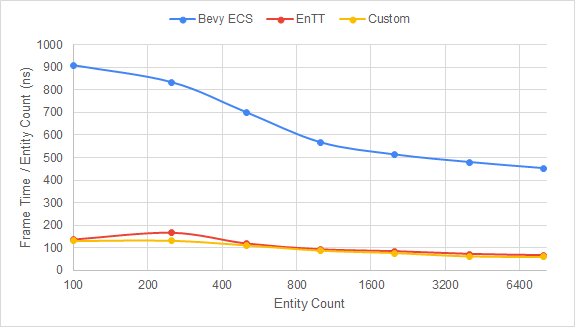
\includegraphics[width=0.4\textwidth]{chart4}}
        \caption{Benchmark~\ref{subsec:structural-changes}: Scatter plot detailing frame time per entity at varying entity count.}
        \label{fig:chart4}
    \end{figure}

    \begin{table}[htbp]
        \caption{Benchmark~\ref{subsec:structural-changes} – Statistics}
        \begin{center}
            \begin{tabular}{|c|c|c|c|c|c|}
                \hline
                \textbf{Entity} & \textbf{ECS} & \multicolumn{4}{|c|}{\textbf{Frame Time (microseconds)}} \\
                \cline{3-6}
                \textbf{Count} & \textbf{Framework} & \textbf{Mean} & \textbf{\textit{Std.Dev.}} & \textbf{\textit{Min}} & \textbf{\textit{Max}} \\
                \hline
                100            & Bevy               & 82.519        & 9.150                      & 57                    & 200                   \\
                & EnTT               & 13.731        & 0.854                      & 10                    & 19                    \\
                & Custom             & 13.989        & 0.566                      & 12                    & 17                    \\
                \hline
                250            & Bevy               & 179.518       & 19.655                     & 135                   & 315                   \\
                & EnTT               & 34.865        & 3.283                      & 28                    & 70                    \\
                & Custom             & 38.707        & 4.854                      & 30                    & 78                    \\
                \hline
                500            & Bevy               & 335.878       & 38.078                     & 235                   & 680                   \\
                & EnTT               & 60.377        & 4.629                      & 48                    & 108                   \\
                & Custom             & 62.21         & 7.509                      & 48                    & 120                   \\
                \hline
                1000           & Bevy               & 580.667       & 58.969                     & 440                   & 1333                  \\
                & EnTT               & 96.754        & 9.943                      & 77                    & 221                   \\
                & Custom             & 103.315       & 12.867                     & 85                    & 218                   \\
                \hline
                2000           & Bevy               & 1044.088      & 75.280                     & 811                   & 1836                  \\
                & EnTT               & 160.129       & 16.238                     & 122                   & 314                   \\
                & Custom             & 161.302       & 16.706                     & 145                   & 420                   \\
                \hline
                4000           & Bevy               & 2024.916      & 120.372                    & 1656                  & 3230                  \\
                & EnTT               & 280.599       & 23.471                     & 218                   & 448                   \\
                & Custom             & 264.531       & 19.182                     & 227                   & 480                   \\
                \hline
                8000           & Bevy               & 3853.080      & 168.052                    & 3188                  & 4967                  \\
                & EnTT               & 510.233       & 48.307                     & 395                   & 935                   \\
                & Custom             & 509.261       & 59.871                     & 396                   & 1298                  \\
                \hline
            \end{tabular}
        \end{center}\label{tab:results-benchmark-4}
    \end{table}

    \paragraph*{Executable Size and Memory Usage}Table~\ref{tab:results-size-and-memory} shows the executable size and memory usage of the frameworks while running the workload according to the given scenarios.
    The size of the executable did not particularly change as each benchmark's configurations varied, while memory usage scaled linearly.
    As such, only one configuration of each scenario sufficed for display.
    We observe that the custom framework-built executable size was approximately 25\% the size of the equivalent EnTT-built executable (except for~\ref{subsec:structural-changes}, where it was around 16.1\%,) while the Bevy-built executable size is substantially higher.
    The simple explanation was that Bevy housed not just the ECS, but also various other features designed to support application development.
    Reducing Bevy from the overall engine to the parts relevant to the Bevy ECS would decrease executable size, but not by enough of a margin to contend with the other frameworks.

    Regarding memory usage, EnTT consumed the least memory, followed by the custom framework, then Bevy.
    As Bevy ECS is part of a broader engine ecosystem, the additional functionalities, such as change detection,
    scheduling infrastructure, metadata, and registries are likely to contribute to the larger memory footprint.
    Considering the other frameworks, the custom framework may have used more complex data storage
    and temporary objects compared to EnTT, such as the structured query objects, thereby contributing to more memory usage.

    \begin{table*}
        \caption{Executable Size and Memory Usage of ECS Frameworks in Benchmark Scenarios}
        \begin{center}
            \begin{tabular}{|c|c|c|c|c|c|c|}
                \hline
                \textbf{Scenario} & \multicolumn{3}{|c|}{\textbf{Executable Size (KB)}} & \multicolumn{3}{|c|}{\textbf{Memory Usage (MB)}} \\
                \cline{2-7}
                & Bevy  & EnTT & Custom & Bevy & EnTT & Custom \\
                \hline
                Benchmark~\ref{subsec:entity-iteration}                & 28097 & 179  & 42     & 9.4  & 3.4  & 8.5    \\
                64K Entity Count                                       &       &      &        &      &      &        \\
                \hline
                Benchmark~\ref{subsec:sparse-access}                   & 28102  & 168  & 44     & 6.0  & 1.7  & 3.4    \\
                0.20 Sparse Ratio                                      &       &      &        &      &      &        \\
                \hline
                Benchmark~\ref{subsec:entity-creation-and-destruction} & 28092  & 188  & 41     & 2.8  & 0.7  & 0.9    \\
                1K Entity Rate                                         &       &      &        &      &      &        \\
                \hline
                Benchmark~\ref{subsec:structural-changes}              & 28149  & 298  & 48     & 4.6  & 0.9  & 1.3    \\
                1K Entity Count                                        &       &      &        &      &      &        \\
                \hline
            \end{tabular}
        \end{center}
        \label{tab:results-size-and-memory}
    \end{table*}


    \section{Limitations}
    \label{sec:limitations}

    A limitation of this evaluation is that the implementations were compiled using different toolchains.
    Since Bevy itself is an engine written in Rust, its build process is entirely different from the C++ implementations.
    Moreover, compiler-specific optimizations may significantly influence the measured performance in addition to the design of the ECS framework.
    This choice was made because our implementation targeted an existing MSVC-based game project,
    and attempts to build it using MinGW resulted in undefined behavior.
    With Bevy also being built in a different language, the reported performance behavior should be interpreted as
    comparisons between complete framework implementations, rather than compiler-independent measurements.
    The evaluation was also run on only one hardware configuration.
    This may result in device-specific artifacts that may interfere with the evaluation, such as other running processes.

    Regarding the evaluation method, the measurements of memory usage with Task Manager can also be seen to be imprecise compared to more sophisticated methods like the Resource Monitor.
    This meant that the results should be taken as broad trends, not precise measurements of component-storage memory usage.
    The single-run benchmark scenarios that create entities with randomized component data may also result in variance between runs that were not captured in the recorded run, and repetitions may not be sufficient to capture the variance of ECS performance.
    Further, these benchmark systems are crafted specifically to fully utilize the ECS for a specific type of workload.
    While this is appropriate for performance evaluation, they do not represent complete simulations or applications with tens of systems running in tandem.

    The EnTT implementation used standard view-based iteration.
    EnTT also provides owned groups, which reorganize component storage to improve iteration locality
    for frequently accessed component combinations.
    These optimizations were not evaluated as part of this benchmark.
    Consequently, the results should be interpreted as representative of the tested view-based implementation
    rather than the theoretical maximum performance achievable with EnTT\@.
    Similarly, the Bevy implementation used the entire Bevy crate with minimal plugins as the standard.
    Any additional optimizations, such as conditional running or events, were not evaluated.


    \section{Discussion and Conclusion}
    \label{sec:conclusion}

    This paper set out to examine the potential of compile-time specialization to imrpove the performance of ECS implementations.
    A custom-built C++ implementation applying compile-time component storage, query type inference, and system registration
    was developed to apply these compile-time optimizations and be used as a reference in the benchmarking process.
    While the results did not imply a universal performance advantage, it revealed promising insights for ECS development and usage.

    The benchmarking data demonstrated that the custom implementation showed strong performance for entity iteration while remaining
    competitive for entity creation and destruction when compared to the two selected frameworks.
    However, it showed weaker performance for sparse access.
    In all scenarios, it delivered smaller executables while exhibiting a somewhat higher memory usage than EnTT.

    The chosen sparse-set storage was beneficial for the custom framework for structural changes and entity lifecycle handling.
    However, it was also evident with Bevy's performance at higher entity counts the advantage of archetype storage for dense iteration scenarios.
    While compile-time query and system specialization reduced some overhead, the costs of sparse lookup could not be eliminated.
    As a result, the choice of storage architecture may have dominated the workload performance at higher entity scenarios.

    In terms of the executable size, the results showed that the custom executable was substantially smaller.
    This may indicate that compile-time specialization had removed the general-purpose runtime infrastructure of the ECS,
    leaving behind generated code that took the form of pure functions.
    The comparison with Bevy could not be said to be equivalent, however, as Bevy included broader engine functionalities.

    In terms of memory usage, we observe somewhat of a trade-off between executable size and runtime memory.
    The custom framework used more memory than EnTT in the reported scenarios, so compile-time specialization did not necessarily minimize the runtime footprint further.

    All in all, in conclusion, the results suggest that extensive compile-time specialization can produce performance competitive
    with established ECS frameworks for standard iteration and structural workloads, but its benefits come from coupling it
    with optimized storage, query building, and system execution policy.

    \bibliographystyle{IEEEtran}
    \bibliography{refs}

\end{document}
